\documentclass{beamer}
\usetheme[subsectionpage=progressbar, background=white]{metropolis}
\usepackage[utf8]{inputenc}
\usepackage{graphicx,color}
\usepackage{amsfonts}
\usepackage{amsmath}
\usepackage{amssymb}
\usepackage{verbatim}
\usepackage{fancyhdr}
\usepackage{epigraph}
\usepackage{caption}
\usepackage{psfrag}
\usepackage{afterpage}
\usepackage[backend=biber, style=nature]{biblatex}
\addbibresource{../bibTex/thesis-library.bib}
\useinnertheme{circles}
\graphicspath{{../figures/}}



\title{Nanoscale hydrodynamics near solids}
\date{June 2019}
\author{Diego Duque Zumajo}
\institute{Departamento Física Fundamental \\Universidad Nacional de Educación a Distancia}

% logo of my university
\titlegraphic{%
\begin{picture}(0,0)
\put(308,-119){\makebox(0,0)[rt]{
\includegraphics[width=1.5cm]{logo}}}
\end{picture}}

\begin{document}
\maketitle

\begin{frame}
\frametitle{Agenda}
\tableofcontents
\end{frame}


\section{Introduction}
\begin{frame}{Roadmap}
  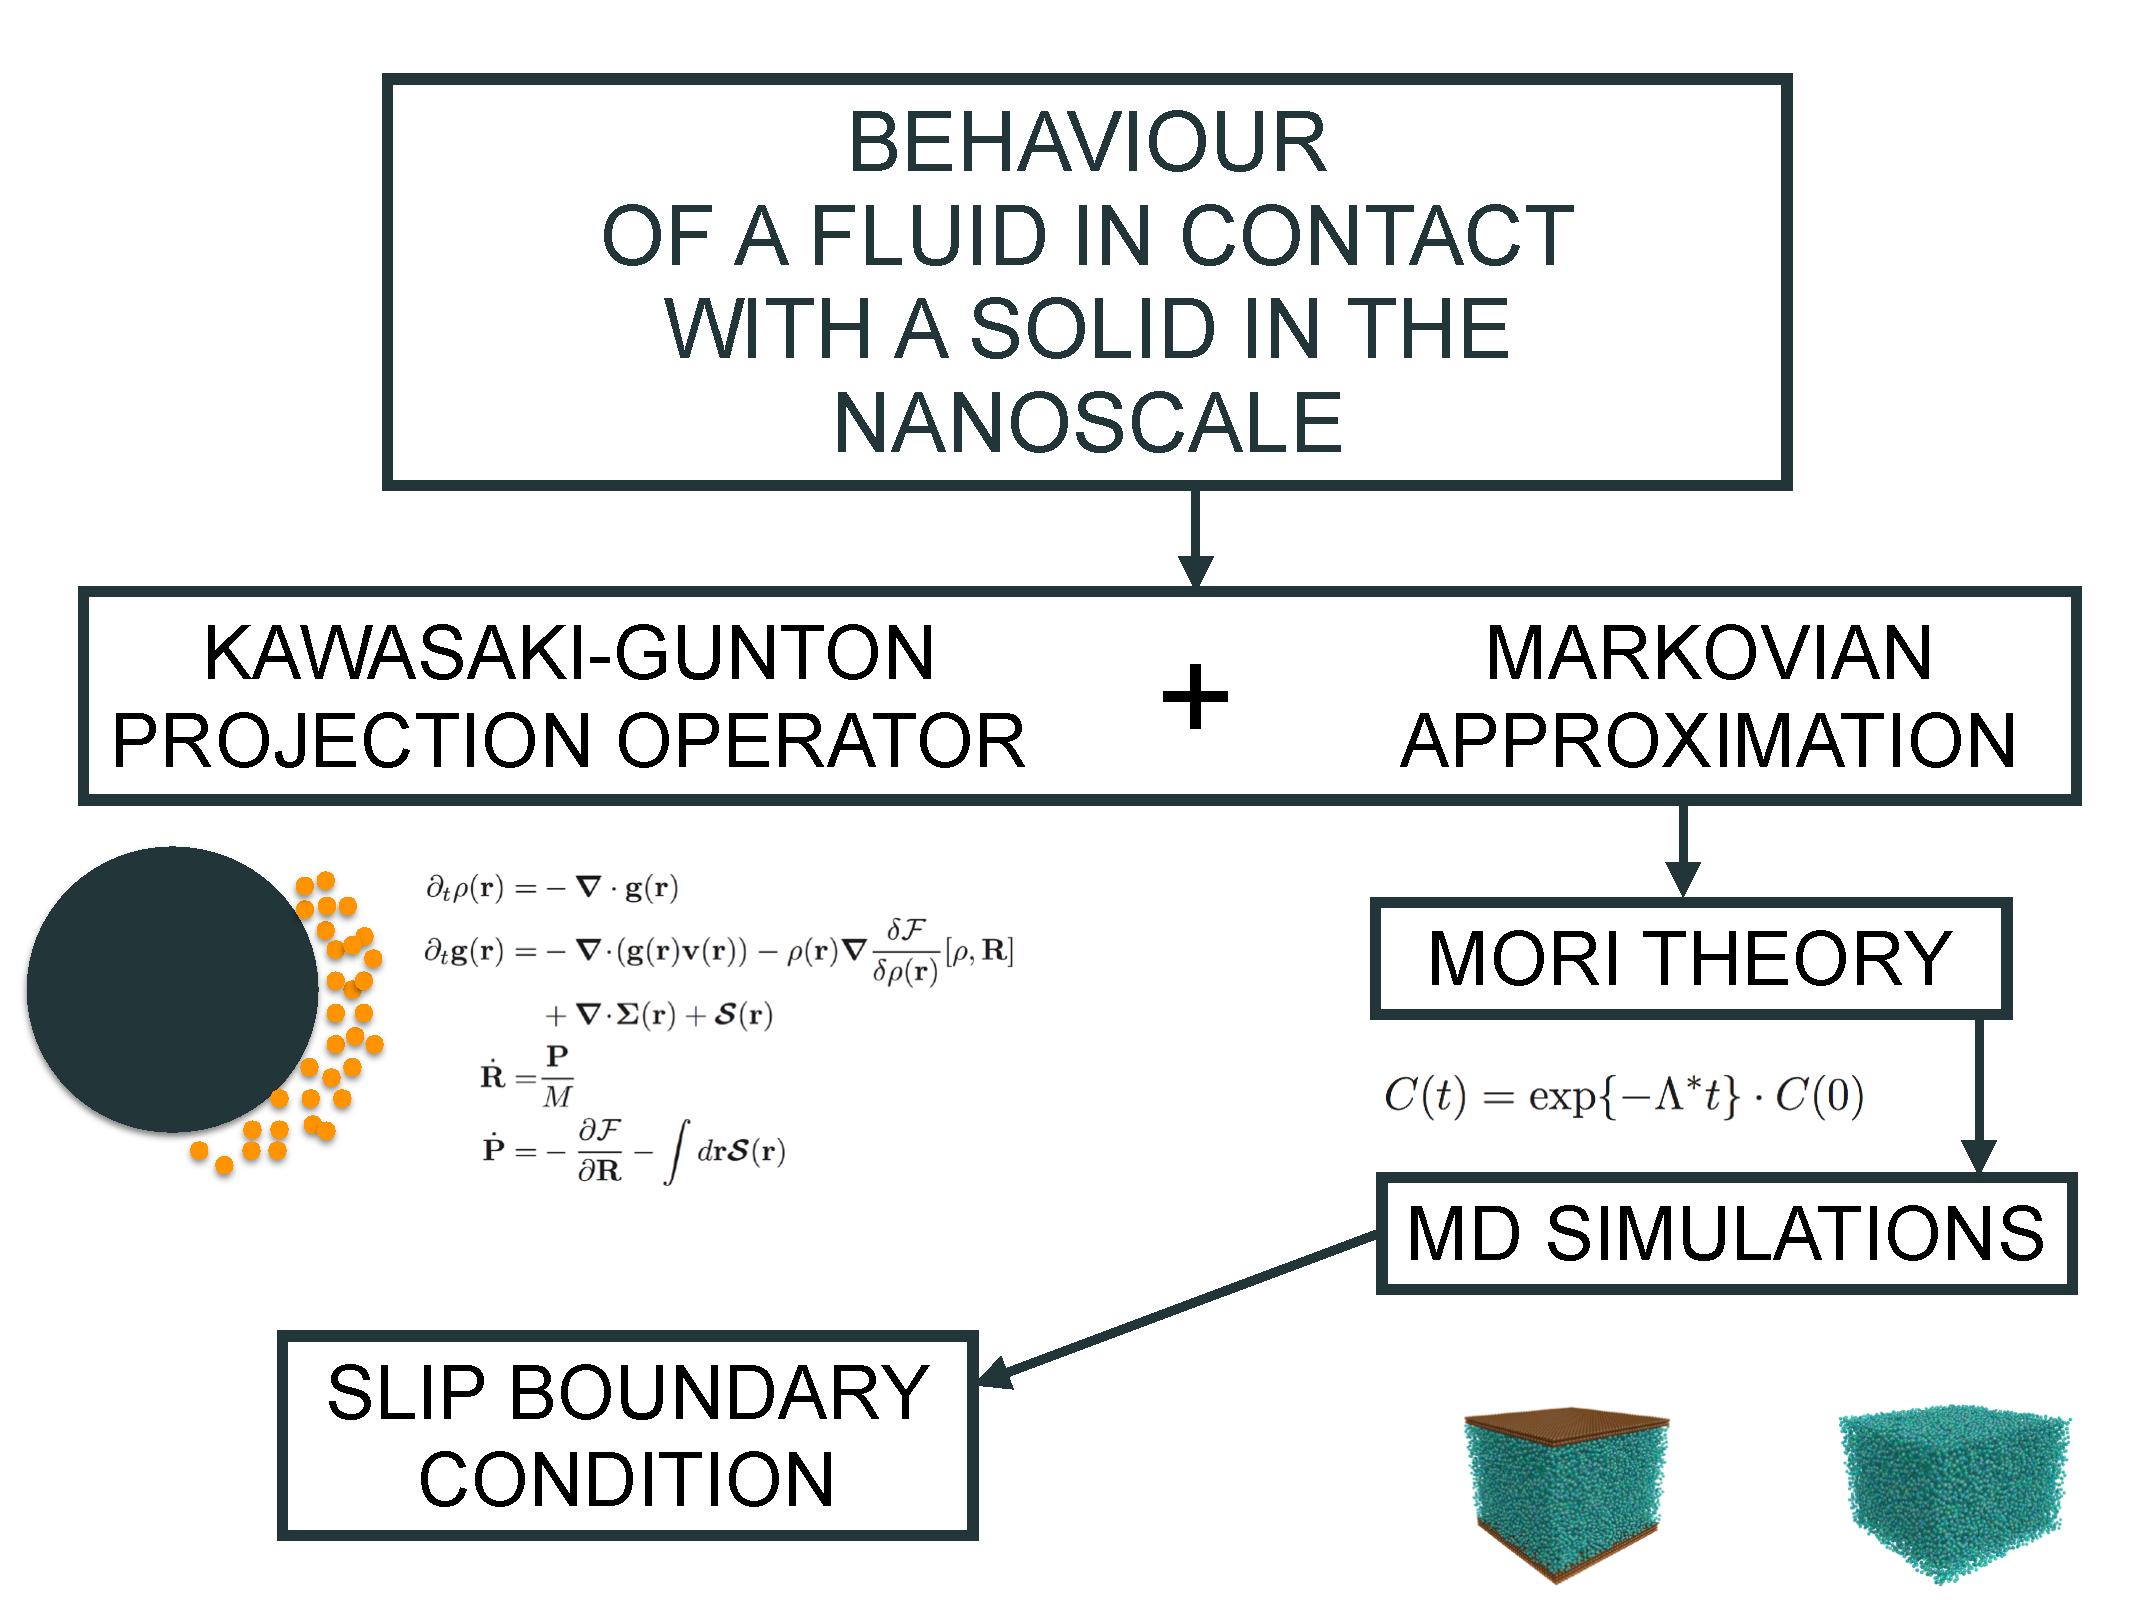
\includegraphics[width=\linewidth]{scheme-thesis}

\end{frame}
\begin{frame}{Roadmap}
  \begin{enumerate}
    \item The study of \alert{the behaviour of a fluid in contact with a solid} in the nanoscale. 
    \item Theory of Coarse-Graining in order to obtain the equations of motion of a fluid in contact with a huge solid sphere.
    \item To address the plateau problem.
    \item MD simulations. 
    \item Mori theory 
  \end{enumerate}
\end{frame}

\begin{frame}{Derivation of the slip boundary condition from NESM}
\begin{itemize}
\item Through the  measurement of the correlation of
the  transverse  momentum  and  comparison  with  the  predictions  of
continuum  (local) hydrodynamics  \cite{Bocquet1993,Chen2015}.
\item Through
linear  response theory  relating  the  force on  the  walls with  the
velocity   of  the   fluid   \cite{Bocquet1993,Petravic2007}.
\item By formulating  linear,  in  general  non-Markovian,  conections  between
friction forces and velocities \cite{Hansen2011}, where the meaning of
this quantities is often understood implicitly.
\end{itemize}
\end{frame}

\begin{frame}{The Theory of Coarse-Graining}
\end{frame}

\begin{frame}{CG variables}
\end{frame}

\begin{frame}{The entropy}
\end{frame}

\begin{frame}{The dynamics}
\end{frame}

\begin{frame}{The Kawasaki-Gunton projection operator}
\end{frame}

\begin{frame}{Mori's Generalized Langevin equation}
\end{frame}

\section{Nanoscalehydrodynamics theory for liquids near solids}
\begin{frame}{Overview}
\end{frame}

\begin{frame}{The system and the CG variables}
\end{frame}

\section{Nanoscale hydrodynamics for planar geometries}
\begin{frame}{Simpler theory}
  Simple theory
\end{frame}

\section{Nanoscale hydrodynamics for unconfined fluids}
\begin{frame}{The system}
  \includegraphics[width=.5\linewidth]{temp_wo_walls}
\end{frame}
\begin{frame}{The system}
  \includegraphics[width=.5\linewidth]{temp_wo_walls_w_layers2}
\end{frame}

\section{NonMarkovian behaviour}
\begin{frame}{Nonmarkovian}
Texto
\end{frame}
\begin{frame}{The system}
  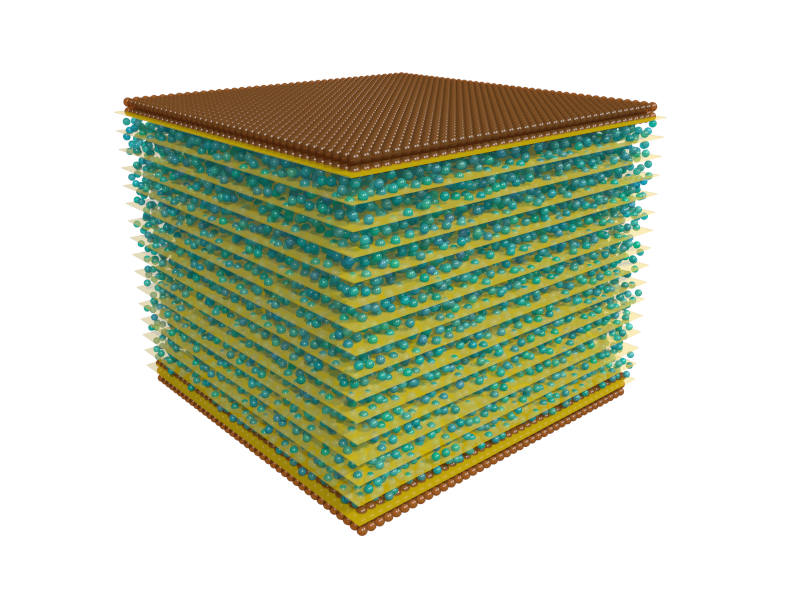
\includegraphics[width=.5\linewidth]{PRL3_gold2_wo_diffuse}
\end{frame}

\section{Conclusions and future directions}
\begin{frame}{Conclusions}
\end{frame}
\begin{frame}{Future directions}
\end{frame}

\section{Relevant references}
\begin{frame}{References}
\end{frame}
\begin{frame}{}
  \centering
  Muchas gracias
  
\includegraphics[width=2.5cm]{logo}
\end{frame}

\end{document}
